\documentclass{acm_proc_article-sp}

\usepackage{multirow}
\usepackage{rotating}
\usepackage{graphicx}
\usepackage{url}
\usepackage{hhline}
\usepackage[utf8]{inputenc}
\usepackage[english]{babel}
\usepackage{eurosym}
\usepackage[pdftex]{color}

\newfont{\mycrnotice}{ptmr8t at 7pt}
\newfont{\myconfname}{ptmri8t at 7pt}
\let\crnotice\mycrnotice%
\let\confname\myconfname%

\begin{document}

\long\def\symbolfootnote[#1]#2{
\begingroup
\def\thefootnote{\fnsymbol{footnote}}\footnote[#1]{#2}
\endgroup}

\def\sharedaffiliation{\end{tabular} \begin{tabular}{c}}

\conferenceinfo{ACM SAC}{'15 Salamanca, Spain}
\CopyrightYear{2015} % Allows default copyright year (2000) to be over-ridden - IF NEED BE.
\crdata{0-12345-67-8/90/01}  % Allows default copyright data (0-89791-88-6/97/05) to be over-ridden - IF NEED BE.

\title{Predicting Well-Being With Geo-Referenced Data Collected from Social Media Platforms}

% --- Author Metadata here ---
\permission{Permission to make digital or hard copies of all or part of
this work for personal or classroom use is granted without fee provided 
that copies are not made or distributed for profit or commercial advantage 
and that copies bear this notice and the full citation on the first page. 
Copyrights for components of this work owned by others than the author(s) 
must be honored. Abstracting with credit is permitted. To copy otherwise, 
or republish, to post on servers or to redistribute to lists, requires 
prior specific permission and/or a fee. Request permissions from Permissions@acm.org.}
\conferenceinfo{SAC'15}{April 13 - 17 2015, Salamanca, Spain\\
{\mycrnotice{Copyright is held by the owner/author(s). Publication rights licensed to ACM.}}}
\copyrightetc{ACM \the\acmcopyr}

\crdata{978-1-4503-3196-8/15/04\ ...\$15.00.\\ http://dx.doi.org/10.1145/2695664.2695939}
% --- End of Author Metadata ---

\numberofauthors{3}
\author{
\alignauthor João Loff\\ 
\alignauthor Manuel Reis\\ 
\alignauthor Bruno Martins\\ 
\sharedaffiliation
\affaddr{INESC-ID -- Instituto Superior T\'{e}cnico, University of Lisbon} \\
\affaddr{TagusPark, Av. Professor Cavaco Silva, 2744-016 Porto Salvo, Portugal} \\
\affaddr{\email{\normalsize \{joao.loff,manuel.barreto.reis,bruno.g.martins\}@tecnico.ulisboa.pt} }
}

\date{}

\maketitle

\begin{abstract}
This paper proposes a novel method that leverages geo-referenced social media data, together with human assessments of particular words, to estimate population well-being across the U.S. territory. We specifically attempt to learn linear regression models that, by leveraging on simple features that essentially correspond to word counts in lexicons of emotionally-charged words, are capable of approximating a composite well-being index built through traditional surveying methods. Experiments with a large Twitter dataset collected within the year of 2012 attest for the feasibility of the proposed approach (i.e., we approximate the Gallup-Healthways composite well-being index with a mean absolute error of 0.91), and we then produced choropleth maps, either at a state- or at a
county-level of detail, that show how well-being varies across the continental U.S. territory.
\end{abstract}

\category{H.4.m}{Information Systems Applications}{Miscellaneous}

\terms{Measurement, Theory, Verification}

\keywords{Applications of Geo-referenced Social Media, Text-Driven Forecasting, Community Well-Being}

\section{Introduction}

Social media data has proven to be remarkably useful for tracking geographical variations of interest to many different topical areas, including public health~\cite{Paul:2011:Tweets,Culotta:2014:ECH:2611105.2557139}, politics and ideology~\cite{Smith:2010:Tweets}, neighborhood deprivation and racial segregation~\cite{Quercia:2013:UCG:2487788.2488000}, demography~\cite{Adnan:2013:Tweets}, marketing~\cite{Gopinath:2014:Tweets}, language usage~\cite{Mocanu:2013:Tweets}, and sociolinguistics in general~\cite{Eisenstein:2011:DSA:2002472.2002641}.

This paper concerns with the usage of geo-referenced data, collected from social media platforms like Twitter, to estimate a population-level well-being index at specific geographic regions. Population well-being essentially refers to how people evaluate their lives in terms of cognition (i.e., general life satisfaction) and emotion (i.e., feeling positive and negative emotions), and the concept has been widely studied in the psychological literature~\cite{Diener:2000:Well-Being,Mackerron12}. Well-being has also been tracked by governmental agencies and by private surveying organizations, such as Gallup-Healthways.

However, survey research is expensive in terms of time and resources. We would like to find faster and cheaper methods to assess life satisfaction, that can help in the study of factors that contribute to well-being, and that can support fine-grained spatial and temporal scales.  Ongoing research initiatives such as the the Hedonometer\footnote{\url{http://www.hedonometer.org}} project or the World Well-Being\footnote{\url{http://wwbp.org/}} project, among others, have started to look at social media to study variations in happiness and other psychological states~\cite{Quercia:2012:TGC:2145204.2145347,Schwartz:2013:Tweets,Dodds:2011:Tweets,Bertrand:2013:Tweets}. The research reported in this paper goes further in this direction, given that we propose to use linear regression to estimate population well-being in the continental U.S. territory (i.e., excluding the states of Alaska and Hawaii), with basis on features derived from Twitter messages containing words that are known to be associated to specific psychological states.

We collected approximately 500,000 geo-referenced tweets from the year of 2012, afterwards mapping the geospatial coordinates that are associated to the tweets into the corresponding U.S. states and counties. Our specific data collection methodology was different from that of previous studies in the area~\cite{Schwartz:2013:Tweets}, in the sense that we collected a small percentage of messages that are directly geo-referenced into specific coordinates (i.e., messages typically issued through mobile devices), instead of relying on heuristics to disambiguate the location field in user profiles. While a different methodology might have given us access to a larger dataset, we preferred to avoid the geocoding noise related to the unreliability of the location field within user profiles~\cite{Hecht:2011:TJB:1978942.1978976}.

Using our Twitter dataset, we then attempted to leverage the words used in the tweets in order to predict well-being, as measured in the corresponding U.S. states through traditional surveys. We specifically matched the words that appear in the tweets against psychology constructs such as the Affective Norms for English Words (ANEW) lexicon~\cite{Bradley1999ANEW}, in order to compute descriptive features that capture information related to affective language use in the different geographic regions. We then use these features in a linear regression model, which combines them in order to approximate a composite well-being index. We relied on the composite well-being index, produced by Gallup-Healthways\footnote{\url{http://info.healthways.com/wbi2013}} for the year of 2012, as ground-truth U.S. state-level well-being information. Through leave-one-out cross-validation, we trained and evaluated linear regression models that attempt to approximate this specific index, on the basis of features that essentially correspond to word counts in lexicons of emotionally-charged words. We also propose to visualize the results through choropleth maps, which show how well-being varies across the continental U.S. territory, either at a state-level or at a county-level of detail.

\section{Methodology}

Our study essentially concerns with attempting to approximate, for each state in the continental U.S. territory and for the year of 2012, a composite well-being index that has been produced by Gallup-Healthways through traditional surveying methods. The Gallup-Healthways 2012 index was based on U.S. nationwide telephone interviews with 1.000 individuals seven days a week, excluding only the major holidays. The interviews examined Americans’ perceptions on topics such as physical and emotional health, healthy behaviors, work environment, social and community factors, financial security, and access to necessities such as food, shelter and healthcare. We attempted to predict the well-being overall score given in the individual state-level reports. The 2012 national average for the well-being overall score was of 66.5 in 100.0, and results ranged from a high of 69.4 in 100.0 (Colorado) to a low of 61.3 in 100.0 (West Virginia).

To build our estimation model, we propose to leverage on Twitter data, collected also from the year of 2012, and on previously available direct human assessments of emotionally-charged words. We specifically relied on the human assessments that are available from two specific lexicons that have been used in related studies, namely the Affective Norms for English Words (ANEW) lexicon~\cite{Bradley1999ANEW}, and a larger English lexicon, produced through a crowdsourcing methodology, that has been made available in the context of the hedonometer project~\cite{Dodds:2011:Tweets}. Previous studies have already shown that these lexicons are adequate to fashion measurement instruments that have a sufficient sensitivity to be of use in evaluating and discriminating texts~\cite{Dodds:2010:Lyrics,Dodds:2011:Tweets}.

ANEW is based on a tri-dimensional perspective of emotions, providing affective norms in terms of valence (which ranges from pleasant to unpleasant), arousal (which ranges from calm to excited), and dominance (ranging from in control to out of control), for a small set of words that had been previously identified as bearing meaningful emotional content. Participants in the original ANEW study used a 1–9 point scale, with half integer increments, to grade their reactions to a set of 1034 English words, including verbs, nouns, and adjectives, with respect to the three aforementioned standard semantic differentials. The ANEW lexicon associates words to the average responses given by the participants in the study. As for the hedonometer lexicon, also referred to as LabMT, it is instead based on a single dimension of happiness, associating numerical estimates collected from human evaluators through Amazon’s Mechanical Turk service, also on a 1–9 point scale, to a total of 10,222 frequently used English words~\cite{Dodds:2011:Tweets}.

Using the aforementioned lexicons, and for each Twitter message, we can compute an average score for the semantic dimensions of valence, arousal, dominance, and happiness, by taking the average value of the scores that are associated to each lexicon word that also appears in the tweet. For instance, to estimate the overall valence score for a given Twitter message, which we denote by $v_{tweet}$, we (i) determine the frequency $f_i$ that the $i$th word from the the ANEW lexicon appears in the text, and then (ii) compute a weighted average of the valence of the ANEW study words as shown below, where $v_i$ is the recorded average valence for word $i$ within ANEW. A similar approach can be used in the case of other lexicons and semantic dimensions.
\begin{equation}
v_{tweet} = \frac{\sum_{i=1}^n v_i \times f_i}{\sum_{i=1}^n f_i}
\end{equation}
Using these average values (i.e., the average scores of all Twitter messages) we then represent geospatial regions (i.e., the different states in the continental U.S. territory, excluding Alaska and Hawaii, or the corresponding counties for each state) according to the following set of features:

\begin{figure*}[t!]
\centering
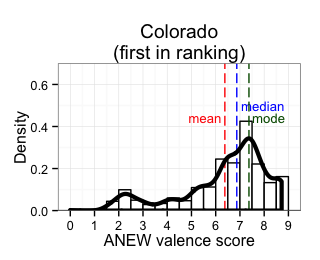
\includegraphics[width=0.22\textwidth]{tweets_distribution_anew_colorado}
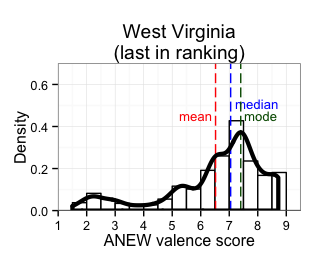
\includegraphics[width=0.22\textwidth]{tweets_distribution_anew_west_virginia}
~~~
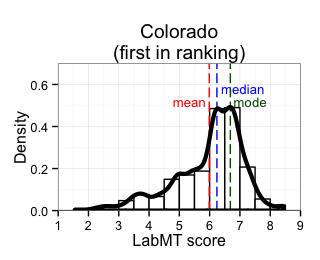
\includegraphics[width=0.22\textwidth]{tweets_distribution_hedonometer_colorado}
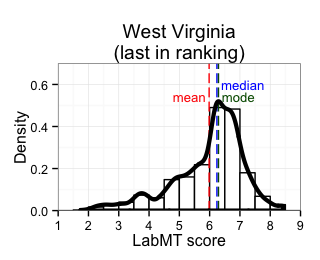
\includegraphics[width=0.22\textwidth]{tweets_distribution_hedonometer_west_virginia}

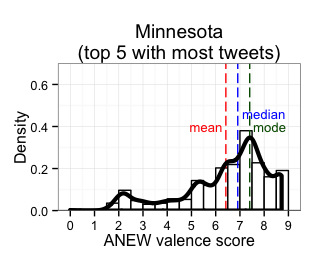
\includegraphics[width=0.22\textwidth]{tweets_distribution_anew_minnesota}
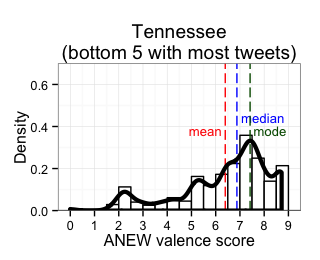
\includegraphics[width=0.22\textwidth]{tweets_distribution_anew_tennessee}
~~~
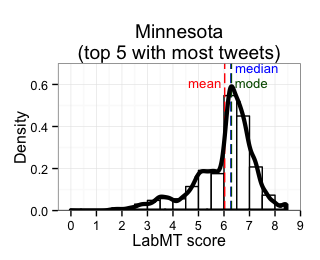
\includegraphics[width=0.22\textwidth]{tweets_distribution_hedonometer_minnesota}
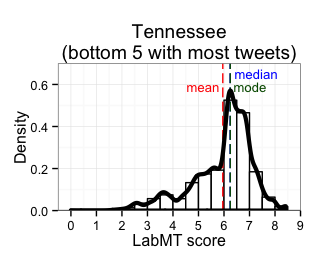
\includegraphics[width=0.22\textwidth]{tweets_distribution_hedonometer_tennessee}
\caption{Distribution for the average ANEW valence scores (the charts on the left) and for the average hedonometer happiness scores (the charts on the right), across all Twitter messages of particular states.}
\label{f1}
\end{figure*}

\begin{itemize}
\item The minimum, maximum, mean, median, mode, and standard deviation in the average happiness scores, computed for each geo-referenced Twitter message that is known to be associated to the state/county, through the hedonometer lexicon;
\item The minimum, maximum, mean, median, mode, and standard deviation in the average happiness scores, again computed through the hedonometer lexicon, but only considering words whose average happiness lies within the interval $7 < h_{avg} \leq 9$, in an attempt to highlight the positive elements of the messages.
\item The mean, median, mode, and standard deviation in the average happiness scores, also computed through the hedonometer lexicon, but after excluding neural words whose average happiness lies within a delta of 1 from the neutral score of 5;
\item The minimum, maximum, mean, median, mode, and standard deviation in the average valence scores, computed for each Twitter message through a similar approach to that of the first set of features, but this time using the entire ANEW lexicon;
\item The minimum, maximum, mean, median, mode, and standard deviation in the average arousal scores, also computed for each Twitter message through ANEW;
\item The minimum, maximum, mean, median, mode, and standard deviation in the average dominance scores, also computed for each Twitter message through the usage of the entire ANEW lexicon;
\item The absolute number, and the percentage of Twitter messages collected for the region (i.e., the state or the county), that contain words in the ANEW lexicon;
\item The absolute number, and the percentage of Twitter messages collected for the region, that contain words in the the entire hedonometer lexicon, that contain words with an average happiness between $7 < h_{avg} \leq 9$, and that contain non-neutral words from this same lexicon;
\item The average number of ANEW words per Twitter message in the region (i.e., the state or the county);
\item The average number hedonometer words per Twitter message in the region, the average number of non-neutral hedonometer words, and also the average number of words whose average happiness lies within the interval $7 < h_{avg} \leq 9$;
\end{itemize}

In the first six feature types from the previous enumeration, and noticing that the average scores that are inferred for each message, with basis on lexicons, are continuous values in the range from 1-9, the mode is computed as the value at which the corresponding density function has its maximum value. A total of 46 features is thus computed for each region (e.g., for each continental U.S. state), and these features are then used for training a linear regression model.

Figure~\ref{f1} illustrates the distribution for the average ANEW valence scores, as well as for the hedonometer average happiness scores, as computed from each Twitter message associated to the states of Colorado and West Virginia (i.e., respectively the states having the highest and lowest values in the Gallup-Healthways index). Besides these two states, and noticing that the volume of Twitter messages available for each state can have an impact on the distributions, Figure~\ref{f1} also illustrates the results for the state with the highest volume of Twitter messages that is ranked in the top-5 states according to the Gallup-Healthways index (i.e., Minnesota), and for the state in the bottom-5 of the ranking that has the highest volume of messages (i.e., Tennessee). Notice that the different measures for the central tendency of the distributions have relatively similar values in all four cases, although the distributions themselves are somewhat different. Notice also that the actual volume of messages with high valence/happiness scores is higher in the case of states that rank first in the Gallup-Healthways index.

Using the aforementioned features for each state in the continental U.S. territory, and using also the ground-truth information for each state in the Gallup-Healthways composite well-being index, we then learned a linear regression model with state-of-the-art Elastic Net regularization, to predict well-being over the continental U.S. states.

Considering a dataset \{${y_i, x_{i1},...,x_{ik}\}^n_{i=1}}$ with $n$ instances (i.e., one for each state that is considered for model training), and assuming that the relationship between the dependent variable $y_i$ (i.e., the composite well-being index) and the $k$-vector of features $x_i$ is linear, we have that a linear regression model takes the following form:
\begin{equation*}
\scriptstyle \begin{pmatrix}
y_1\\y_2\\\cdots\\y_n
\end{pmatrix} =
\begin{pmatrix}
1 & x_{11} & \cdots & x_{k1}\\
1 & x_{12} &  \cdots & x_{k2}\\
\cdots & \cdots & \cdots & \cdots\\
1 & x_{1n} & \cdots & x_{kn}
\end{pmatrix} \times
\begin{pmatrix}
b_0 \\ b_1 \\ b_2 \\ \cdots \\ b_k
\end{pmatrix} +
\begin{pmatrix}
e_1 \\ e_2 \\ \cdots \\ e_n
\end{pmatrix}
\end{equation*}
In the formula, $x_{ij}$ corresponds to the $i$-th feature of the $j$-th instance, the $b_i$ parameters correspond to the regression coefficients, and $e_j$ is an error that captures the difference between the actual observed responses $y_i$, and the prediction outcomes of the regression model. In a matrix notation form, we have that $y = Xb + e$. Zou and Hastie proposed the Elastic Net approach for regularizing Linear Least Squares Regression (LSR) models, that combines $l_1$ and $l_2$ regularization penalties with weights $\lambda_1$ and $\lambda_2$, respectively~\cite{elasticNet}. The estimates for the parameters $b$ given by the Elastic Net method are defined by the following optimization problem:
\begin{equation*}
b = \operatorname*{\arg\min}_b  ||y - Xb||^2 + \lambda_1||b||_1 + \lambda_2||b||_2^2
\end{equation*}
For finding the model parameters, we used the implementation based on cyclical coordinate descent from the glmnet package for the R system for statistical computing~\cite{elasticNet2}. When reporting predictions, we threshold the results produced by the regression models to the interval 0-100.

Lastly, using the results produced by the regression model, we attempted to build map-based visualizations that illustrate the variation in well-being across the U.S. continental territory. We used the R system for statistical computing to produce choroplet maps from the well-being estimates, similar to those that are included in the original Gallup-Healthways well-being reports.

\begin{figure}[b!]
\centering
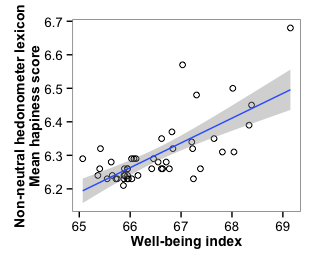
\includegraphics[width=0.23\textwidth]{scatter_1}
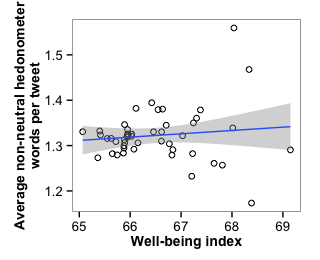
\includegraphics[width=0.23\textwidth]{scatter_2}
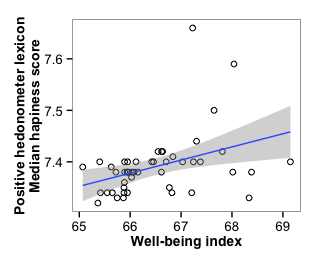
\includegraphics[width=0.23\textwidth]{scatter_3}
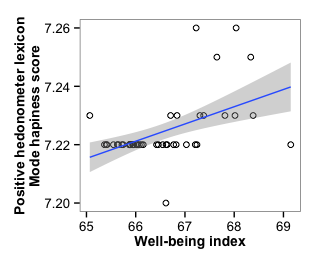
\includegraphics[width=0.23\textwidth]{scatter_4}
\caption{Correlation between the most informative features, and the values of the well-being index.}
\label{f2}
\end{figure}

\section{Results}

For evaluating the proposed approach in terms of the quality of the approximations to the well-being index produced by Gallup-Healthways, we leveraged a leave-one-out cross-validation methodology, in which all except one of the considered U.S. states are used for training the regression model, which is then evaluated in the remaining state. This procedure is repeated for all states, and we finally report on the quality of the obtained results through the Mean Absolute Error (MAE) and Root Mean Square Error (RMSE) metrics. The obtained results in our cross-validation experiment correspond to a MAE of 0.92 and a RMSE of 1.22. A simple baseline approach, based on assigning to all the states the average value for the Gallup-Healthways well-being index, would lead to a MAE of 1.40 and a RMSE of 1.73.

We also measured the Peason $\rho$ and Kendall $\tau$ correlation coefficients between the estimates produced through our regression models, and the ground-truth results from the Gallup-Healthways index. The obtained results correspond, in this case, to the values of $\rho=0.7441$ and of $\tau=0.5862$. Most states are indeed associated to similar positions when ranking them according to either our estimates or the ground-truth index. The states for which the ranking differences are more extreme are Maryland and Minnesota. The reader should also note that Pearson correlations between behavior (i.e., language use) and psychologically based variables rarely exceeds an $\rho$ of 0.4~\cite{Meyer2001}, and both these values correspond to higher results than those reported on previous related studies~\cite{Schwartz:2013:Tweets,Mitchell:2013:Tweets}.

The regression coefficients obtained by averaging the results from the different cross-validation folds show that, of the 46 features that were considered, only 28 have a non-zero value (i.e., remember that the Elastic Net regularizer attempts to shrink the coefficients of the less relevant features towards zero). The most discriminative feature was found to be the mode of the happiness score obtained from the filtered version of the hedonometer lexicon, that only considered non-neutral words. Most of the features with positive values in the estimated regression coefficients were obtained from the hedonometer lexicon. Some features obtained from the ANEW lexicon, such as the minimum and standard deviation on the valence scores, or the mode of the dominance scores, were associated to small negative values in the estimated regression coefficients. In Figure~\ref{f2}, we plot the correlation between the 4 features that have the highest values in terms of the estimated regression coefficients, and the values from the Gallup-Healthways composite well-being index.

Figure~\ref{f3} presents, side by side, two choropleth maps corresponding to the state-level composite well-being scores that are estimated through our models, or that are available as part of our ground-truth. In order to facilitate the comparison, we present results in terms of quintiles (i.e., we divided the well-being scores into 5 essentially equal-sized subsets), instead of directly showing the well-being scores associated to the different states. The raw data used for building these visualizations is detailed in Table~\ref{t1}, which also shows per-state values associated to the number of tweets collected for the state, the number of tweets containing words in either the ANEW or the hedonometer lexicons, and the average values for the valence, happiness, arousal and dominance dimensions. According to our models, the 2012 national average for the well-being index is of 66.5 in 100.0, and results range from a high of 69.15 in 100.0 (Colorado) to a low of 65.07 in 100.0 (West Virginia).

\begin{figure*}[t!]
\centering
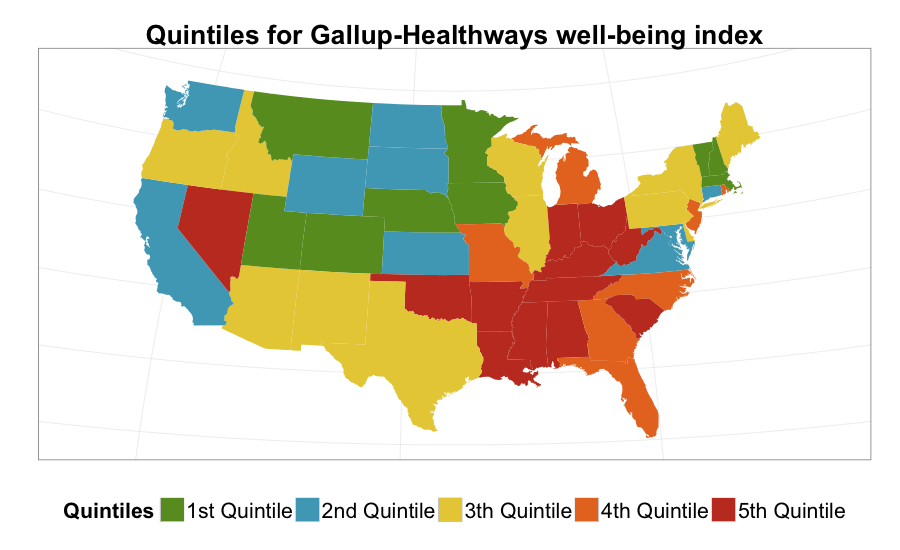
\includegraphics[width=0.48\textwidth]{quintiles_state_gallup_2}
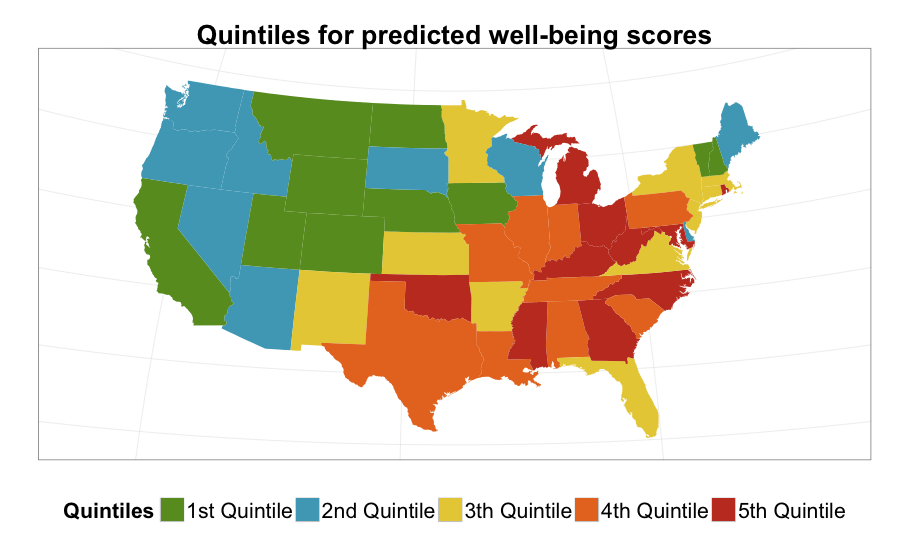
\includegraphics[width=0.48\textwidth]{quintiles_state_model}
\caption{Per-state well-being in continental U.S. according to the reports by Gallup-Healthways (map on the left) and according to our regression models (map on the right).}
\label{f3}
\end{figure*}

Figure~\ref{f4} instead presents a choropleth map corresponding to county-level composite well-being, computed through the same general methodology, but in this case using a regression model that was fitted to the entire dataset with the ground-truth information for the different U.S. states, instead of using cross-validation folds. The areas shown in grey correspond to counties for which we where unable to collect Twitter messages containing words from the considered lexicons, and most of these counties are associated to states with high values in the well-being index.

\begin{figure}[b!]
\centering
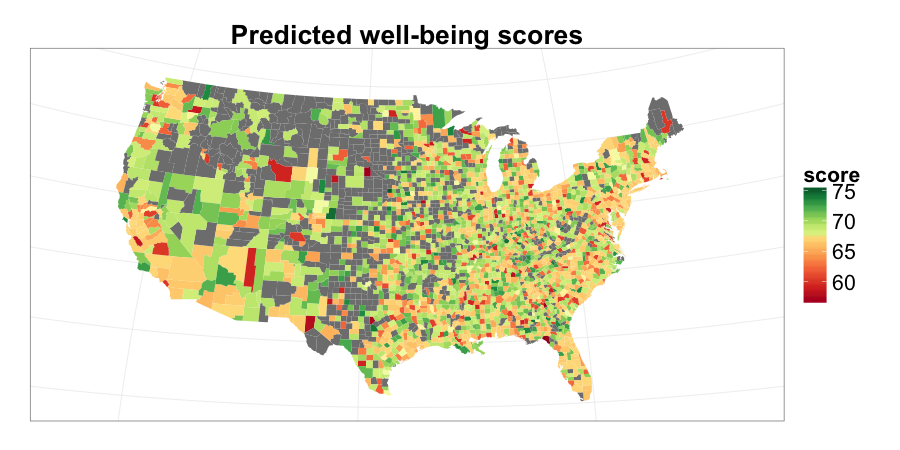
\includegraphics[width=0.49\textwidth]{scores_by_county_model}
\caption{Per-county well-being in the continental U.S. territory, according to our regression model.}
\label{f4}
\end{figure}

\section{Related Work}

Measuring public well-being is a key task for researchers and policymakers alike, and several researchers have noted that public sentiment and mood can be quantified using Twitter and other related Internet sources. The current explosion of available social media data offers the promise of a much more time-sensitive and geographically specific analysis of population-level well-being.

For instance in the context of the hedonometer project, researchers have explored both the dynamics and geography of happiness, as expressed over Twitter messages~\cite{Dodds:2011:Tweets,Mitchell:2013:Tweets,Frank:2013:Tweets}. These authors used Amazon's Mechanical Turk service to quantify the happiness of individual English words, and they then estimate an average happiness scores from sets of messages collected from Twitter’s gardenhose feed. Through this relatively simple instrument, the authors have analyzed temporal and geographical variations in happiness, and they have also correlated highly-resolved demographic characteristics with happiness levels. The authors also showed that the happiness scores, estimated through their method, correlate well with well-being indexes produced through surveys (i.e., the authors report on a correlation $\rho = 0.511$ against the Gallup-Healthways index for the year of 2011~\cite{Mitchell:2013:Tweets}).

\begin{table*}[t!]
\begin{center}
\scriptsize
\begin{tabular}{l c c c c c c c c c c }
	          & Gallup- & Predicted  & Number       & With ANEW      & With LabMT   & Average & Average    & Average & Average   \\
State         & Healthway & Well-Being & of Tweets    & Words & Words & Valence & Happiness  & Arousal & Dominance \\
\hline
\hline
Alabama        & 64.2 & 65.949 & 7373 & 2226 & 6432 &  6.33 & 5.54 & 5.31 & 5.54 \\
Arizona        & 67.1 & 66.637 & 6463 & 2166 & 5960 &  6.44 & 5.55 & 5.50 & 5.63 \\
Arkansas       & 64.1 & 66.027 & 2936 & 921 & 2677 &  6.25 & 5.56 & 5.26 & 5.51 \\
California     & 67.4 & 67.243 & 41199 & 11674 & 36900 &  6.41 & 5.47 & 5.39 & 5.59 \\
Colorado       & 69.7 & 69.148 & 2428 & 767 & 2143 &  6.38 & 5.53 & 5.38 & 5.61 \\
Connecticut    & 67.6 & 66.074 & 4342 & 1326 & 3888 &  6.37 & 5.52 & 5.34 & 5.59 \\
Delaware       & 66.6 & 66.821 & 2185 & 649 & 1972 &  6.21 & 5.53 & 5.24 & 5.45 \\
Florida        & 65.8 & 66.033 & 26984 & 8852 & 24741 & 6.37 & 5.51 & 5.38 & 5.57 \\
Georgia        & 66.1 & 65.868 & 32100 & 9802 & 29358 & 6.21 & 5.50 & 5.27 & 5.49 \\
Idaho          & 67.1 & 67.227 & 334 & 126 & 302 & 7.24 & 5.58 & 5.75 & 6.14 \\
Illinois       & 66.6 & 65.892 & 15682 & 4599 & 13977 & 6.32 & 5.51 & 5.38 & 5.57 \\
Indiana        & 65.1 & 65.949 & 8746 & 3080 & 8026 & 6.44 & 5.54 & 5.44 & 5.60 \\
Iowa           & 68.1 & 67.812 & 3062 & 786 & 2627 & 6.40 & 5.45 & 5.39 & 5.53 \\
Kansas         & 67.6 & 66.115 & 2298 & 781 & 2041 & 6.28 & 5.54 & 5.33 & 5.55 \\
Kentucky       & 62.7 & 65.402 & 6098 & 1877 & 5524 & 6.28 & 5.51 & 5.41 & 5.54 \\
Louisiana      & 64.7 & 65.947 & 9239 & 2747 & 8207 & 6.31 & 5.48 & 5.30 & 5.54 \\
Maine          & 67.3 & 66.840 & 535 & 200 & 495 & 6.04 & 5.53 & 5.18 & 5.38 \\
Maryland       & 68.0 & 65.746 & 17163 & 4887 & 15269 & 6.28 & 5.48 & 5.34 & 5.52 \\
Massachusetts  & 68.1 & 66.423 & 8336 & 2786 & 7483 & 6.30 & 5.52 & 5.36 & 5.55 \\
Michigan       & 65.6 & 65.650 & 15426 & 4524 & 13945 & 6.26 & 5.52 & 5.31 & 5.54 \\
Minnesota      & 68.9 & 66.459 & 4537 & 1469 & 4150 & 6.42 & 5.55 & 5.38 & 5.59 \\
Mississippi    & 63.6 & 65.365 & 8130 & 2408 & 7367 & 6.14 & 5.48 & 5.25 & 5.44 \\
Missouri       & 65.5 & 65.878 & 6351 & 1941 & 5772 & 6.27 & 5.51 & 5.33 & 5.54 \\
Montana        & 68.5 & 68.336 & 177 & 69 & 161 & 6.25 & 5.42 & 5.47 & 5.58 \\
Nebraska       & 68.5 & 67.304 & 1334 & 456 & 1234 & 6.43 & 5.57 & 5.40 & 5.60 \\
Nevada         & 65.2 & 66.618 & 4069 & 1360 & 3613 & 6.59 & 5.56 & 5.50 & 5.68 \\
New Hampshire  & 68.4 & 67.648 & 687 & 195 & 607 & 6.34 & 5.56 & 5.35 & 5.58 \\
New Jersey     & 66.1 & 65.964 & 16688 & 5172 & 15054 & 6.28 & 5.54 & 5.32 & 5.52 \\
New Mexico     & 66.7 & 66.548 & 1398 & 432 & 1314 & 6.34 & 5.51 & 5.32 & 5.57 \\
New York       & 66.2 & 66.614 & 20671 & 6565 & 18235 & 6.30 & 5.52 & 5.31 & 5.54 \\
North Carolina & 65.7 & 65.548 & 18227 & 5727 & 16659 & 6.28 & 5.52 & 5.29 & 5.52 \\
North Dakota   & 67.4 & 68.016 & 545 & 223 & 511 & 6.03 & 5.48 & 5.39 & 5.47 \\
Ohio           & 64.6 & 65.720 & 20011 & 6189 & 18351 & 6.29 & 5.53 & 5.37 & 5.57 \\
Oklahoma       & 65.2 & 65.628 & 3173 & 1006 & 2859 & 6.17 & 5.52 & 5.33 & 5.50 \\
Oregon         & 67.1 & 66.708 & 2189 & 736 & 1974 & 6.45 & 5.56 & 5.39 & 5.59 \\
Pennsylvania   & 66.5 & 65.941 & 19932 & 6353 & 18013 & 6.34 & 5.53 & 5.34 & 5.58 \\
Rhode Island   & 65.5 & 65.416 & 1128 & 389 & 1046 & 6.02 & 5.49 & 5.41 & 5.47 \\
South Carolina & 65.2 & 65.887 & 9420 & 3097 & 8614  & 6.27 & 5.49 & 5.29 & 5.51 \\
South Dakota   & 68.0 & 67.210 & 600 & 149 & 497 & 6.38 & 5.50 & 5.33 & 5.59 \\
Tennessee      & 64.0 & 65.890 & 8065 & 2574 & 7306 & 6.39 & 5.55 & 5.34 & 5.61 \\
Texas          & 66.6 & 65.878 & 44317 & 13964 & 40371 & 6.21 & 5.50 & 5.36 & 5.50 \\
Utah           & 68.8 & 67.380 & 1863 & 682 & 1715 & 6.34 & 5.52 & 5.36 & 5.51 \\
Vermont        & 68.6 & 68.039 & 137 & 59 & 129 & 6.66 & 5.59 & 5.56 & 5.69 \\
Virginia       & 67.7 & 66.153 & 14886 & 4487 & 13294 & 6.33 & 5.53 & 5.31 & 5.55 \\
Washington     & 67.7 & 67.030 & 3575 & 1212 & 3303 & 6.42 & 5.56 & 5.38 & 5.62 \\
West Virginia  & 61.3 & 65.068 & 1781 & 585 & 1622 & 6.52 & 5.57 & 5.41 & 5.69 \\
Wisconsin      & 67.3 & 66.770 & 5357 & 2290 & 4941 & 5.83 & 5.49 & 4.68 & 5.26 \\
Wyoming        & 67.9 & 68.385 & 246 & 95 & 230 & 5.86 & 5.53 & 5.16 & 5.21 \\
\hline
Average        & 66.5 & 66.504 & 9009 & 2805 & 8144 & 6.32 & 5.52 & 5.35 & 5.55 \\
Minimum        & 61.3 & 65.068 & 137 & 59 & 129 & 5.83 & 5.42 & 4.68 & 5.21 \\
Maximum        & 69.7 & 69.148 & 44317 & 13964 & 40371 & 7.24 & 5.59 & 5.75 & 6.14 \\
\hline
\end{tabular}
\end{center}
\caption{Well-being results for the different states in the continental U.S. territory.}
\label{t1}
\end{table*}

Bertrand et al. reported on building a public sentiment map of the Manhattan and surrounding areas according to the analysis of over 600,000 tweets, organized by census block~\cite{Bertrand:2013:Tweets}. The authors developed a classifier that uses key words, phrases and emoticons to determine the mood of each tweet (i.e., the authors used supervised learning to train a classifier, where messages are represented through words and phrases, and where the training data corresponds to messages where the positive and negative labels are determined by the presence of particular emoticons). Leveraging their classifier and a large collection of geo-referenced Twitter messages, the authors built maps that aggregate public sentiment according to census blocks.

Quercia et al. considered Twitter users based in a variety of London census communities, studying the relationship between sentiment expressed in tweets and community socio-economic well-being, as reported in the 2007 UK government’s Index of Multiple Deprivation~\cite{Quercia:2012:TGC:2145204.2145347}. For classifying the individual tweets, the authors compared a word counting technique based on computing the standardized difference between the percent of words that are known to reflect a positive sentiment, and those that are known to reflect a negative sentiment, against a second approach based on a sentiment classifier implemented through a maximum entropy model. The authors showed that the results of these two methods correlate and are reasonably accurate, and they also showed a significant correlation between Twitter sentiments and well-being (i.e., the higher the normalized sentiment score of a community’s tweets, the higher the community’s socio-economic well-being).

The work that is perhaps more similar to ours is that of Schwartz et al.~\cite{Schwartz:2013:Tweets} in the context of the World Well-Being project, in which the authors also attempted to predict well-being across the U.S. territory, with basis on Twitter data. The authors collected a billion tweets from June 2009 to March 2010, and mapped most of them to U.S. counties by geocoding the location field associated to the Twitter users posting the messages. Using a Lasso regularized linear regression model, they then correlated the words used in the tweets (in the form of LDA-generated word topics, or through the usage of hand-build lexicons) with population well-being, as measured through surveys for 2009 and 2010. The authors also had access to county-level demographic information (i.e., age, sex, and ethnicity) and indicators of socio-economic status (i.e., income and education) from the U.S. census, which they used as controls in their predictive models. The authors found that word use gives additional predictive accuracy above the socio-demographic controls, and they also showed visualizations of the word topics that better predict population well-being. The results also support many of the patterns that have been observed in the well-being literature, including positive effects of prosocial activities, exercise, engagement at school and work, and openness to and engagement with life.

\section{Conclusions and Future Work}

This paper proposed the usage of linear regression to estimate population well-being in the continental U.S. territory, with basis on features derived from Twitter messages containing words that are known to be associated to specific psychological states. Experiments with a large Twitter dataset collected from the year of 2012 attest for the feasibility of the proposed approach (i.e., we approximate the Gallup-Healthways composite well-being index with a mean absolute error of 0.92, and with a Pearson product-moment correlation coefficient of $\rho=$0.7441).

Despite the interesting results, there are also several ideias for future work. For instance our experimental methodology can perhaps be improved, by considering correction methods in the computation of correlation coefficients that can account with the issue spatial autocorrelation. Moreover, given that our general idea is to leverage Twitter data to gauge societal well-being, without depending on traditional surveying methods, we still would have to see if indeed the regression models that are learned with data from particular year(s) (e.g., Twitter messages from 2012, in our case) would generalize to approximating well-being also to other years (i.e., see if the same models, when provided with features that reflect Twitter contents for the subsequent years of 2013 and 2014 would still produce accurate approximations). Although research on whether search or social media can predict real-world quantities has actually become commonplace, many recent studies have also highlighted the fact that the quality of stand-alone monitors, built from social media data, can be somewhat questionable~\cite{Lazer14Science,Daniel14Meta}.

Similarly to previous work within the hedonometer project, we would also like to experiment with applying our regression model, capable of approximating well-being, to Twitter messages collected across different timescales (e.g., measuring population well-being at different days of the week or during particular periods of the year) or associated to specific topics (e.g., looking only at messages that are associated to particular hashtags). In the same line, we would also like to apply our methodology to Twitter messages collected for other regions of the world, particularly considering that lexicons such as ANEW have been adapted Spanish~\cite{ANEWES}, Portuguese~\cite{ANEWPT}, and other languages.

For future work, and in this case similarly to the previous research reported by Schwartz et al.~\cite{Schwartz:2013:Tweets}, we would also like to experiment with the usage of regression models that use the entire vocabulary of words, as they occur in Twitter messages, to forecast the well-being index, instead of relying on hand-built lexicons. Regression models built on the entire vocabulary would allow us to better understand specific factors contributing to well-being. Finally, and also similarly to Schwartz et al.~\cite{Schwartz:2013:Tweets}, we would like to experiment with the introduction of additional variables (e.g., demographic and socio-economic features, derived from information available from the U.S. census bureau) into our regression models for estimating well-being, in an attempt to correct some of the biases in Twitter towards urban and young populations. Recent research has also established a relationship between remote sensing imagery data and survey-based measures of economic and social phenomena~\cite{Regan2012} and, for future work, it would be interesting to complement our models with features derived from overhead imagery, or even features derived from geo-referenced photo collections.

\section*{Acknowledgements}

This work was partially supported by Fundação para a Ciência e a Tecnologia (FCT), through the project grants with references EXCL/EEI-ESS/0257/2012 (DataStorm research line of excellency), EXPL/EEI-ESS/0427/2013 (KD-LBSN), and PEst-OE/EEI/LA0021/2013 (INESC-ID's associate laboratory multi-annual funding). 

\bibliographystyle{plain}
\small
\bibliography{references}

\end{document}





